\section{Experimental Evaluation}\label{sec:evaluation}

The acting system, the robustness heuristic and the task preparations were implemented directly inside the system \ac{FAPE} \citep{bit-monnotTemporalHierarchicalModels2016a}.
The statements that \ac{FAPE} supports acting \citep{dvorakPlanningActingTemporal2014,bit-monnotTemporalHierarchicalModels2016a,bit-monnotFAPEConstraintbasedPlanner2020} do not hold.
The acting implementation is not present in the current version of the system, and the original acting implementation was domain-dependent and only supported non-hierarchical problems.
Additionally, the removal of actions from a chronicle is not implemented, which makes replanning and plan repair impossible.
Lastly, when adding new tasks, they could not create actions during the current plan, as the timeline implementation does not allow splitting timelines to support a new timeline.
Changes to a timeline can only be added before its first or after its last component.
Fixing these issues proved to go beyond the scope of this thesis, however.
The intuitive approach of regarding the planner as a black box and adapting the original problem to include already executed actions creates problems with the hierarchical representation and therefore makes planning impossible.
Evaluation regarding the planning of tasks by interleaving with already planned tasks and replanning is thus done manually.


We evaluate our implementation in three aspects.
First, we compare our hierarchical domain definition to the classical domain definition by \cite{yuxinliuPlanningOvercookedGame2020} in Section \ref{sec:evaluation-htn}.
In Section \ref{sec:evaluation-robustness} we evaluate our robustness heuristic in comparison to the default and makespan heuristic.
Last, we manually evaluate the robustness heuristic and preparations in an acting environment in Section \ref{sec:evaluation-acting}

The evaluation was done in an LXC container with 12 Intel(R) Xeon(R) Gold 6334 CPU 3.60GHz Cores, 32 GB RAM.
Planning in \ac{FAPE} is however a single-threaded process, so only one CPU core can be used.
Each planning iteration was given 1000 seconds to complete.

We consider four different variants of our \textit{Overcooked} domain definition:
\begin{itemize}
  \item Fully hierarchical: All action templates are task-dependent and the duration of the action template \verb|a_move| is fixed at 5.
  \item Fully hierarchical with durations: All action templates are task-dependent and the duration of the action template \verb|a_move| is the shortest distance in the map calculated using the A* search algorithm. 
  \item Partially hierarchical: The action template \verb|a_move| is not task-dependent, so agents can move freely in the domain if necessary and the duration of the action template \verb|a_move| is fixed at 5.
  \item Partially hierarchical with durations: The action template \verb|a_move| is not task-dependent, so agents can move freely in the domain if necessary and the duration of the action template \verb|a_move| is the shortest distance in the map calculated using the A* search algorithm. 
\end{itemize}


% Quantitative Metrics:
% Plan time
% Search Nodes
% Average Branching Factor

% Makespan/Duration

% Qualitative Metrics:
% Success

% Possible Comparisons:
% HTN PO vs HTN TO vs Classical \citep{yuxinliuPlanningOvercookedGame2020}
% HTN vs HTN + Robustness
% HTN Oracle vs HTN Acting vs HTN Acting + Robustness vs HTN + Preparations

\subsection{Environments}

We consider two environments in this evaluation.
The complete environment definition is included in Appendix \ref{app:environments}.


\bild{fig:eval-overcooked}{overcooked2_tutorial}{The tutorial level of ``Overcooked!2''}{10}{``Overcooked!2'' tutorial level}

First, we consider the ``tutorial level'' of the ``Overcooked!2'' game shown in Figure \ref{fig:eval-overcooked}.
The environment provides the three ingredients lettuce, tomato and cucumber, the tableware plate and the tool knife.
The orders that may be received are a simple salad, consisting of only lettuce, a lettuce tomato salad and lastly a salad with lettuce, tomato and cucumber.
All of the ingredients have to be chopped using a knife before they are assembled on a plate.
Each ingredient and tableware is present five times, there are four knives and two cooks available.
The map has a narrow path to get to the locations of the knives.
We define four possible arrange areas, two in the middle on each side and two on the bottom on each side.
We chose this environment, as it contains all of the properties we consider and provides simple to complex tasks.
Also, it is the first environment human players encounter when learning the game, so can serve as an example if the planning system is viable for this domain.

\bild{fig:eval-mapB}{pddl_mapB}{Complex map for making burgers from \cite{yuxinliuPlanningOvercookedGame2020}}{10}{Complex map for making burgers}

Second, we consider the ``complex map'' shown in Figure \ref{fig:eval-mapB} taken from \cite{yuxinliuPlanningOvercookedGame2020}.
This environment is not from the official game but was introduced by them.
It provides the ingredients beef, lettuce, tomato and burger bun, the tableware plate and the tools knife and pan.
The orders received here are burgers with a burger bun, a steak, lettuce and tomato.
The lettuce and tomato have to be chopped and the steak fried in the pan before they are assembled on a plate.
Each ingredient and tableware is again present five times, there are two knives, two pans and two cooks available.
The map has a long counter and cooks must walk around it to move between the ingredient locations and the tools, so the cooks are encouraged to pass ingredients over the counter.
There are two arrange areas at the same place as seen in Figure \ref{fig:eval-mapB}.
This environment provides a more complex recipe and an additional optimization goal with the transportation of ingredients over a counter.

\subsection{HTN vs Classical Planning in \textit{Overcooked}}
\label{sec:evaluation-htn}


In this section, we compare our \ac{HTN} domain definition for \textit{Overcooked} with the \ac{PDDL} domain definition by \cite{yuxinliuPlanningOvercookedGame2020}.
It is not possible to directly compare the makespan between the domains, as not all of the action durations were provided.
To plan using the \ac{HTN} domain definition, we use \ac{FAPE} \citep{bit-monnotTemporalHierarchicalModels2016a} and \cite{yuxinliuPlanningOvercookedGame2020} use the \ac{TFD} planner \citep{eyerichUsingContextenhancedAdditive2009}.
The environment is the ``complex map'' shown in Figure \ref{fig:eval-mapB}.
The goal of this problem is to prepare either one or two burgers.


It is important to note that \ac{FAPE} uses different heuristics by default during planning compared to \ac{TFD}.
\ac{FAPE} uses the heuristic minimal spanning tree for partially hierarchical domains and depth-first search in fully hierarchical domains.
While the selection of different heuristics is possible in \ac{FAPE}, it is not considered in this comparison.
\cite{yuxinliuPlanningOvercookedGame2020} uses the shortest makespan heuristic.
As such, \ac{FAPE} only does satisficing while \ac{TFD} tries to find the optimal plan.

Additionally, \ac{TFD} uses \ac{SSP} while \ac{FAPE} uses \ac{PSP}.
This makes the generated nodes not directly comparable.

The results of planning the delivery of one burger are shown in Table \ref{tab:eval-burger}.
TFD is faster in the generation of the plan and visits significantly more nodes than \ac{FAPE}.
The search time for the partial hierarchy is also slower than the fully hierarchal version.
The inclusion of the representative movement durations also increases the search time for both variants.
The makespan is however shorter for the partial hierarchy compared to the full hierarchy, especially when using the representative movement durations.


\begin{table}
  \centering
  \begin{tabular}{lcllll}
                   & success & search time  & generated nodes & makespan         \\
    \hline
    TFD                & yes & $20s$            &  10546          &  125.1       \\
    Full hier.            & yes & $31.0s\pm 0.9$   & $125\pm 0.0$    &  $232\pm 0.0$            \\
    Full hier. + dur      & yes & $37.9s\pm 1.6$   & $125\pm 0.0$    &  $368\pm 0.0$      \\
    Part. hier.        & yes & $563.0s\pm 45.1$ & $3754\pm 0.0$   &  $227\pm 0.0$   \\
    Part. hier. + dur & yes & $628.0s\pm 16.9$ & $3744\pm 0.5$   &  $318\pm 0.0$            \\
  \end{tabular}
  \caption[Results for producing one burger]{Results of \ac{TFD} and our different domain variations for producing one burger}
  \label{tab:eval-burger}
\end{table}

The results for planning the delivery of two burgers are shown in Table \ref{tab:eval-burgers}.
Both planners are unable to find a solution in this case.
TFD does consider more search nodes than \ac{FAPE}, as in the previous comparison.

\begin{table}
  \centering
  \begin{tabular}{lcllll}
    & success & search time  & generated nodes & makespan         \\
  \hline
  TFD             & no & $1000s+$ & 1000000+ &  -       \\
  Full hier.            & no & $1000s+$ & 5360+    &  -          \\
  Full hier. + dur      & no & $1000s+$ & 7430+    &  -    \\
  Part. hier.       & no & $1000s+$ & 3800+    &  - \\
  Part. hier. + dur & no & $1000s+$ & 3071+    &  -          \\
  \end{tabular}
  \caption[Results for producing two burgers]{Results of \ac{TFD} and our different domain variations for producing two burgers}
  \label{tab:eval-burgers}
\end{table}

\subsection{Robustness Heuristic vs Default and Makespan Heuristics}
\label{sec:evaluation-robustness}

In this section, we evaluate the robustness heuristic introduced in Section \ref{sec:approach-robustness}.
Heuristics can be provided as a list in \ac{FAPE}, to assign a priority.
The additional heuristics are used to break ties between previous heuristics.

The default heuristics of \ac{FAPE} are depth-first search (``dfs''), ordered decomposition (``ord-dec'') and ``soca'' which is a simple comparison between the number of flaws and actions.
We compare this default heuristic with four different combinations of adding either the shortest makespan or the robustness heuristic at index 2 or 3.
The depth-first search should always be at index 1 for fully hierarchical problems, as the search would otherwise not finish in a reasonable timeframe.
We choose $n=m=10$ for the robustness heuristic as a tradeoff between accuracy and feasibility.


We compare the heuristic combinations in the following four different simple problems in the domain variant ``Fully hierarchical with durations''.
This domain is chosen, as the previous evaluation showed that our partially hierarchical domain is not tractable and the durations are relevant for optimizations.
The environment for the salads is the ``tutorial level'' (see Figure \ref{fig:eval-overcooked}).
For the burger it is the ``complex map'' (see Figure \ref{fig:eval-mapB}).
The deadlines are necessary for the robustness heuristic, as it requires some point of failure.
We choose the deadlines for each task such that all tasks can be completed by a single cook in sequence.
\begin{enumerate}
  \item a lettuce salad, with a deadline of 150:\\ 
    \verb|[start, start+150] contains order_lettuce_salad(client1);|
  \item two lettuce salads, with a deadline of 300 each:\\
    \verb|[start, start+300] contains order_lettuce_salad(client1);|\\
    \verb|[start, start+300] contains order_lettuce_salad(client2);|
  \item a tomato salad with a deadline of 200:\\
    \verb|[start, start+200] contains order_lettuce_tomato_salad(client1);|
  \item a burger with a deadline of 400:\\
    \verb|[start, start+400] contains order_lettuce_tomato_burger(client1);|
\end{enumerate}

\begin{table}[t]
\begin{minipage}{\textwidth}
    \begin{center}
      
    \begin{tabular}{p{1.5cm}rrrrr}
    \multicolumn{1}{l}{}         & \multicolumn{1}{l}{heuristic} & success & \multicolumn{1}{l}{plantime} & \multicolumn{1}{l}{generated nodes} & \multicolumn{1}{l}{makespan} \\ \hline \hline
    \multirow{5}{*}{salad}        & default                       & yes     & $11.8s\pm1.5 $              & $46.0\pm0.0$                         & $115.0 \pm0.0$               \\ 
                                  & makespan@2                    & yes     & $11.4s\pm1.5 $              & $53.0\pm0.0$                         & $79.0  \pm0.0$               \\ 
                                  & makespan@3                    & yes     & $11.1s\pm1.7 $              & $53.0\pm0.0$                         & $79.0  \pm0.0$               \\
                                  & robustness@2                  & yes     & $11.6s\pm1.3 $              & $48.6\pm5.3$                         & $110.6 \pm25.5$               \\ 
                                  & robustness@3                  & yes     & $11.7s\pm1.3 $              & $45.8\pm2.5$                         & $115 \pm21.2$               \\\hline
    \multirow{5}{*}{\parbox{1.2cm}{two salads}}   
                                  & default                       & no      & $1000.0s+$                  & $39641.0\pm?$                        & $-     $                     \\
                                  & makespan@2                    & no      & $1000.0s+$                  & $38906.2\pm1541.4$                   & $-     $                     \\
                                  & makespan@3                    & no      & $1000.0s+$                  & $36023.0\pm554.3$                    & $-     $                     \\
                                  & robustness@2                  & no      & $1000.0s+$                  & $16584.0\pm?$                        & $-     $                     \\ 
                                  & robustness@3                  & no      & $1000.0s+$                  & $21336.0\pm?$                        & $-     $                     \\\hline
    \multirow{5}{*}{\parbox{1.5cm}{tomato salad}} 
                                  & default                       & yes     & $10.8s\pm1.5 $              & $75.0\pm0.0$                         & $180.0 \pm0.0$               \\
                                  & makespan@2                    & yes     & $12.0s\pm0.3 $              & $119.0\pm0.0$                        & $118.0 \pm0.0$               \\
                                  & makespan@3                    & yes     & $12.0s\pm0.2 $              & $115.0\pm0.0$                        & $121.0 \pm0.0$               \\
                                  & robustness@2                  & yes     & $15.0s\pm2.7 $              & $171.4\pm39.4$                           & $175.4 \pm2.2$               \\
                                  & robustness@3                  & yes     & $12.1s\pm1.8 $              & $79.2\pm4.3$                            & $190.2 \pm3.9$               \\\hline
    \multirow{5}{*}{burger}       & default                       & yes     & $38.1s\pm 3.1$              & $125.0\pm0.0$                        & $368.0\pm0.0$                \\
                                  & makespan@2                    & no      & $1000.0s+$                  & $5389.2\pm448.1$                     & $-     $                     \\
                                  & makespan@3                    & no      & $1000.0s+ $                 & $5323.6\pm234.7$                     & $-     $                     \\
                                  & robustness@2                  & yes     & $342.1s\pm365.2 $           & $2108.8\pm2462.0$                    & $329.4 \pm21.29$             \\ 
                                  & robustness@3\footnote{The values here are only for the case of success}                  & 40\%    & $28.6s\pm0.8 $    & $71\pm 7.0$                          & $333.0 \pm 8.5$                                      
    \end{tabular}
    \caption[Performance results for different heuristic combinations]{Performance results for different heuristic combinations on different problems. The default heuristic is a priority combination with depth-first search (``dfs''), ordered decomposition (``ord-dec'') and ``soca'' which is a simple comparison between the number of flaws and actions. The other heuristic combinations in the table are created by inserting them at the respective index (starting at 1) in the priority combination, e.g. makespan@2 would result in the list (dfs, makespan, ord-dec, soca).}
    \label{tab:eval-heuristics}
    \end{center}
  \end{minipage}
  \end{table}

The results are shown in table \ref{tab:eval-heuristics}.
Each heuristic variant was evaluated five times on each problem.
The arithmetic mean value is shown first and the standard deviation second.
When the standard deviation is $?$, i.e. unknown, the calculation of the standard deviation returned nan.

Producing a single salad takes only around 10 seconds for all of the heuristics.
The number of generated nodes is similar for all heuristics.
The makespan heuristic combinations achieve a significant decrease in the makespan of the plan.
The makespan of the robustness heuristics is not better than the default and has a high standard deviation.

None of the heuristics can provide a plan for two salads at the same time in under 1000 seconds.
The default and makespan heuristics do however generate more nodes than the robustness heuristics.

All heuristics succeed at planning to prepare the tomato salad, the planning times are between 10 and 15 seconds, with the robustness@2 having the longest mean planning time at 15 seconds.
The highest number of generated nodes has the robustness@2 heuristic, while robustness@3 and the default heuristic generate a similar number of nodes.
The makespan values show a similar picture as when planning for the simple salad.
The makespan heuristics have the shortest makespan value, and the makespan values of the robustness heuristic are not much different than the makespan value of the default heuristic.

The burger is only planned successfully by the default heuristic and the robustness@2 heuristic.
The robustness@3 heuristic succeeds only two out of five times in the 1000 seconds and the makespan heuristics do not finish.
The robustness@2 heuristic has however a very high standard deviation.
The default heuristic generates the lowest number of nodes, while the mean for the robustness@2 heuristic is much higher, but also with a very high standard deviation.
The highest number of nodes are generated by the makespan heuristics, but around seven times fewer nodes than in the two salads problem in the same time frame.
The lowest makespan here is by the robustness@2 heuristic, but again with a high standard deviation.

We now consider one planning result of the robustness@2 for the problem of one tomato salad in detail.
The total makespan of this solution is 161, which is the shortest result for this problem using the robustness@2 heuristic.
The low-level actions that are performed are shown in the following code snippet.
The overall timeline for high-level actions is shown for each cook in Figure \ref{fig:eval-robustness}.

This result shows that the tasks are split between the two cooks.
One prepares the plate, chops and arranges the lettuce and delivers the salad, while the other one chops and arranges the tomato.
Some of the high-level actions like the arranging of the tomato take very long.
The low-level actions reveal that \verb|cook2| remains at \verb|manCounterMiddle2Top| between time 52 and 110, but only places the lettuce on the plate at time 110.
Similarly, \verb|cook1| stands waiting between time 22 and 52 before transporting the lettuce.

\bild{fig:eval-robustness}{robustness-tomato-salad}{High-level actions divided by cook for the task \texttt{order\_tomato\_lettuce\_salad} using the robustness@2 heuristic}{16}{High-level actions for a lettuce tomato salad using the robustness heuristic}

\begin{figure}
  \begin{anmlcode}
  [0,2]     a_move(cook1, manPlateDispenser)
  [0,10]    a_move(cook2, manTomatoDispenser)
  [2,8]     a_pick_up(cook1, plate4)
  [8,18]    a_move(cook1, manCounterMiddle2Top)
  [10,16]   a_pick_up(cook2, tomato1)
  [16,29]   a_move(cook2, manKnife3)
  [18,22]   a_drop(cook1, plate4)
  [29,33]   a_drop(cook2, tomato1)
  [33,44]   a_chop(cook2, tomato1, knife3)
  [45,51]   a_pick_up(cook2, tomato1)
  [51,52]   a_move(cook2, manCounterMiddle2Top)
  [52,65]   a_move(cook1, manLettuceDispenser)
  [65,71]   a_pick_up(cook1, lettuce1)
  [71,87]   a_move(cook1, manKnife4)
  [87,91]   a_drop(cook1, lettuce1)
  [91,102]  a_chop(cook1, lettuce1, knife4)
  [103,109] a_pick_up(cook1, lettuce1)
  [109,122] a_move(cook1, manCounterMiddle2Bottom)
  [110,120] a_arrange(cook2, tomato1, plate4)
  [122,122] a_arrange(cook1, lettuce1, plate4)
  [132,142] a_move(cook1, manCounterMiddle2Top)
  [142,148] a_pick_up(cook1, plate4)
  [148,156] a_move(cook1, manDeliver)
  [156,161] a_give(cook1, client1, plate4)
  \end{anmlcode}
  \captionof{lstlisting}[Low-Level actions for a lettuce tomato salad using the robustness heuristic]{Low-Level actions for the task \texttt{order\_tomato\_lettuce\_salad} using the robustness@2 heuristic}
\end{figure}

\subsection{Acting with Robustness Heuristic or Preparation Insertion}
\label{sec:evaluation-acting}

In this section, we evaluate the impact of the robustness heuristic and the task preparations on acting.
We use the environment ``tutorial level'' in the ``Fully hierarchical with durations'' domain with the following tasks:
\begin{itemize}
  \item \verb|[0,200] contains order_lettuce_tomato_salad(client1);|
  \item \verb|[100,300] contains order_lettuce_tomato_salad(client2);|
  \item \verb|[150,350] contains order_lettuce_tomato_salad(client3);|
\end{itemize}

Each task is received by the activity manager at the start of the temporal interval it is contained in.
We chose the task \verb|order_lettuce_tomato_salad|, as it is more complex than the simple salad and provides enough opportunity for parallelization.
The burger could give a more representative result, but simulating it by hand is not feasible.
The temporal intervals were chosen such that a solution exists, but it is not possible to have each cook fulfill an order sequentially on their own.

We consider four different configurations:
\begin{itemize}
  \item default: no additional changes to \ac{FAPE}
  \item makespan: the makespan@2 heuristic is used to get the shortest plan for each received task.
  \item preparations: the optimal preparations are inserted into the default plan.
  \item robustness: the robustness heuristic is used for generating a plan for each task
\end{itemize}

Acting is simulated using an oracle approach: we manually add the optimal sequence of actions for the second and third tasks consecutively without replanning or repair.
This measures the ability of the configurations to find a plan without replanning or repair.
Since representative action durations are used, the durations for each action may be different.
We therefore use the optimal durations that are calculated with the makespan@2 heuristic for the first task.
These durations are: 
\begin{itemize}
  \item $dur(prep)=20$
  \item $dur(transport)=37$
  \item $dur(chop)=11$
  \item $dur(arrange)=18$
  \item $dur(deliver)=27$
\end{itemize}

The results are shown in Table \ref{tab:eval-acting} and a visual representation is shown in Figure \ref{fig:eval-acting}.
The task \verb|m_chop| was split into the two subtasks \verb|transport| and \verb|a_chop|, as they can be handled by different cooks. 

All of the configurations succeed in this manual evaluation with optimal task addition.
The makespan configuration represents the optimal configuration when not allowing preparations.
It has the highest margin for each task and the highest average margin.
It also has the shortest overall makespan.
The preparations have the second shortest overall makespan.
This configuration has lower margins for each task but a smaller standard deviation for the average margin.
The robustness configuration has a higher margin than the preparations for the first and second tasks but is much lower for task 3.
Therefore the average is a little higher, but the standard deviation is almost doubled.
The total makespan is also only three time steps lower than failure.
The default configuration has the lowest margins and reaches the deadline for task 3 just on time.

\begin{table}
  \centering
  \begin{tabular}{lrrrrrr}
                & success & \multicolumn{3}{c}{margin}  & avg margin     & total makespan  \\
                &         &  task 1 & task 2  & task 3  &                &  \\ \hline
  default       & yes     & $25$    & $32$    &  $0$    & $19\pm16.8$           & $350$     \\
  makespan      & yes     & $87$    & $87$    &  $44$   & $72.7\pm24.8$         & $306$       \\
  preparations  & yes     & $25$    & $42$    &  $16$   & $27.7\pm13.2$         & $323$    \\
  robustness    & yes     & $39$    & $46$    &  $3$    & $29.3\pm23.1$         & $347$ \\
  \end{tabular}
  \caption{Results of the manual acting evaluation}
  \label{tab:eval-acting}
\end{table}



\begin{sidewaysfigure}
  \centering
  \subfloat[Default FAPE, the first transport action only has a smaller height to show that it is overlapping with the arrange action]{\label{fig:eval-acting-default}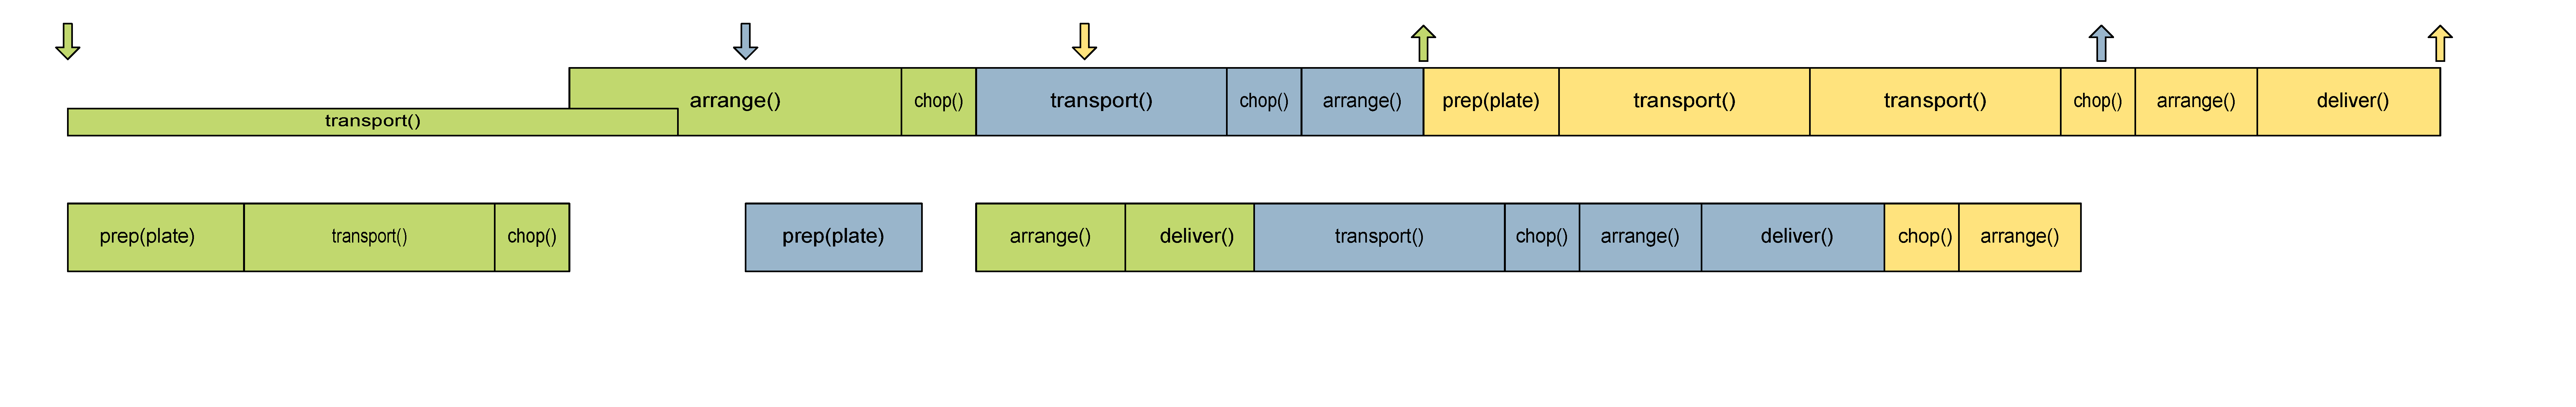
\includegraphics[width=\linewidth]{images/Scenario3 tomato - default.pdf}} \\\medskip
  \subfloat[Makespan heuristic]{\label{fig:eval-acting-makespan}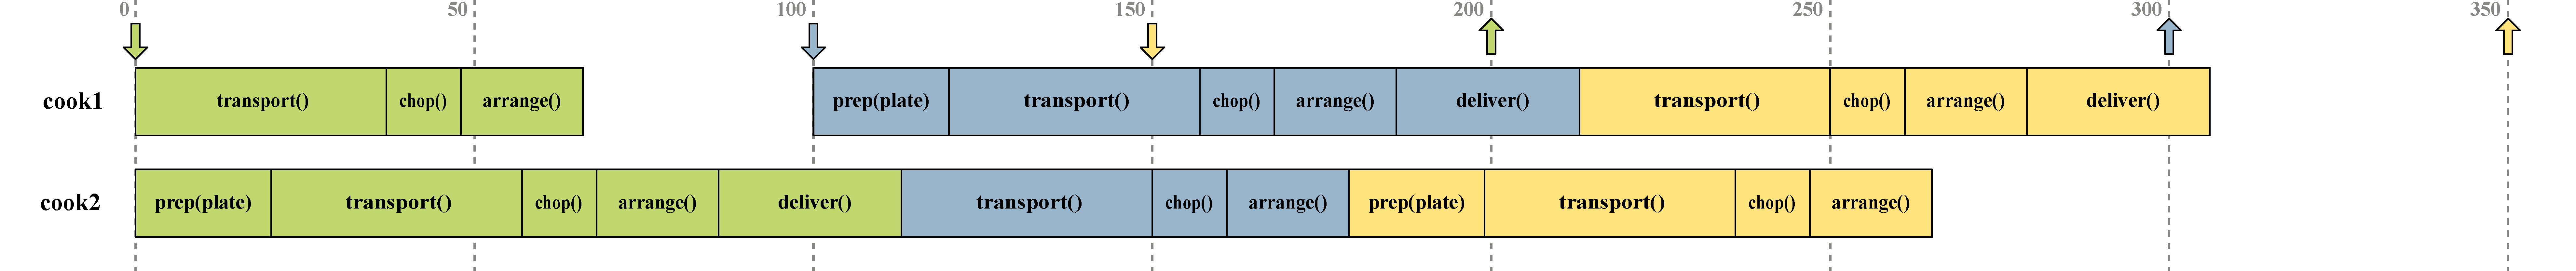
\includegraphics[width=\linewidth]{images/Scenario3 tomato - oracle_makespan.pdf}} \\\medskip
  \subfloat[Preparations, grey boxes represent inserted preparations]{\label{fig:eval-acting-preparations}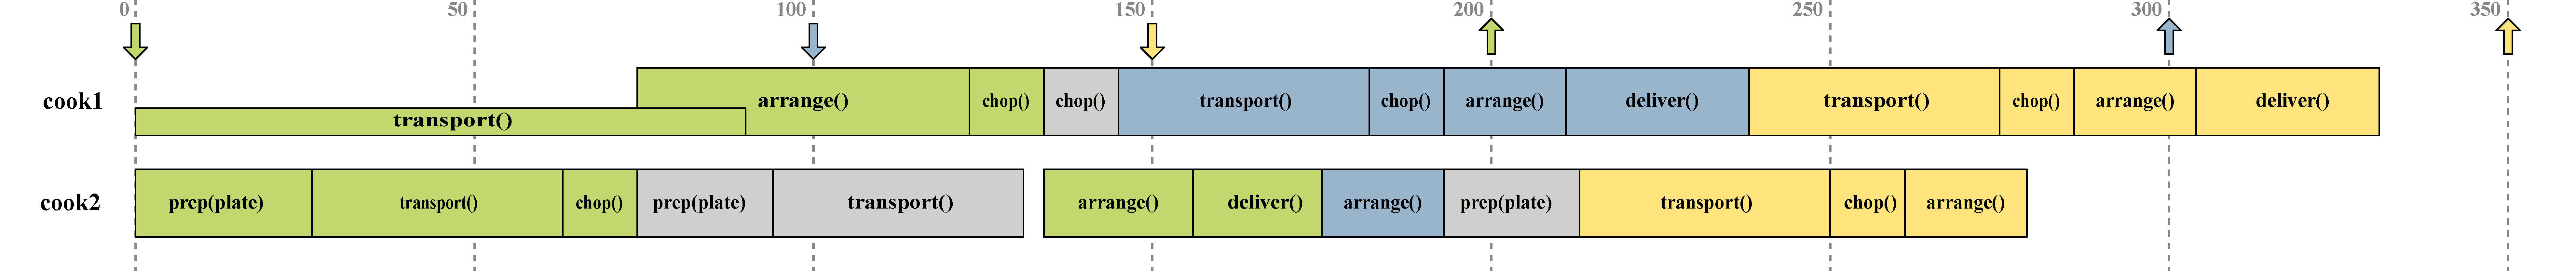
\includegraphics[width=\linewidth]{images/Scenario3 tomato - preparations.pdf}} \\\medskip
  \subfloat[Robustness heuristic]{\label{fig:eval-acting-robustness}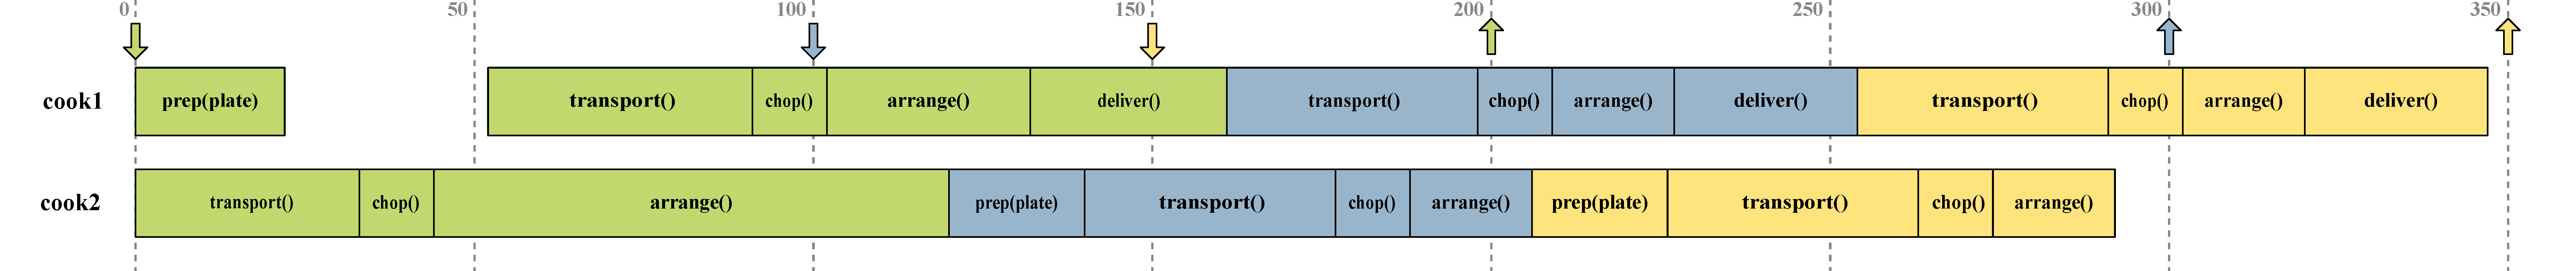
\includegraphics[width=\linewidth]{images/Scenario3 tomato - robustness.pdf}} \\\medskip
  \caption[Timeline-like representations of the acting evaluation]{Timeline-like representations of the plan executed by acting. Each row shows the actions performed by one of the cooks. Each color represents a task, the downpointing arrows represent the start time of a task and the uppointing arrows the deadline.}
  \label{fig:eval-acting}
\end{sidewaysfigure}
